\documentclass{article}
\usepackage{xcolor}
\definecolor{darkgreen}{rgb}{0.0, 0.5, 0.0}
\usepackage[utf8]{inputenc}
\usepackage{graphicx}
\usepackage{subcaption} % Use subcaption instead of subfigure
\usepackage{matlab-prettifier}
\usepackage{amsmath}
\usepackage{pgfplots}
\pgfplotsset{compat=1.18}
% Set equation numbering to section and subsection
%\renewcommand{\theequation}{\thesubsection.\arabic{equation}}
\makeatletter
\@addtoreset{equation}{subsection}
\makeatother
\usepackage{listings}
\usepackage{amssymb}
\usepackage{blindtext}
\usepackage{geometry}
\usepackage{graphicx}
\usepackage{float}
\usepackage{dirtytalk}
\usepackage{enumitem}
\usepackage{derivative}
\usepackage{biblatex}

\usepackage{svg}  % Enables SVG support
\usepackage{hyperref} % Enables hyperlinks
% No red boxes at hyperlinks
\hypersetup{
    colorlinks,
    linkcolor={blue},
    citecolor={blue},
    urlcolor={blue}
}

\lstset{
    language=Python,             % The language of the code
    basicstyle=\ttfamily\small,  % The font style for the code
    keywordstyle=\color{blue},   % Color of Python keywords
    stringstyle=\color{darkgreen},     % Color of strings
    commentstyle=\color{gray},  % Color of comments
    showstringspaces=false,      % Do not show spaces in strings
    frame=single,                % Frame around the code
    numbers=left,                % Line numbers on the left
    numberstyle=\tiny\color{gray},  % Style of the line numbers
    breaklines=true,             % Automatic line breaking
}%Imports biblatex package
 \geometry{
 a4paper,
 total={160mm,250mm},
 left=25mm,
 top=30mm,
 footskip =10mm,
 }

\title{Calculus Uge 4}
\author{Thomas Sejer Canham}
\date{\today} 
\setlength\parindent{0pt}

 \begin{document}

\begin{titlepage}
 \maketitle
 \thispagestyle{empty}
\end{titlepage}
I denne uge skal vi arbejde med planintegraler. Ideen med planintegraler er at vi kan integerere funktioner over et arbitrært område i planet. Jeg vil betegne dette område som $R$. Den uformelle retfærdiggørelse for at vi kan integerere over et arbitrært område er Fubini's sætning. Kort fortalt kan vi definere en hjælpefunktion $f^*(x,y)$ som er lig med $f(x,y)$ hvis $(x,y) \in R$ og 0 ellers. Så kan vi integerere over hele planet og få det samme resultat som at integerere over området $R$.

\begin{equation}
    f^*(x,y) = \begin{cases}
        f(x,y), & \text{hvis } (x,y) \in R \\
        0, & \text{ellers}
    \end{cases}
\end{equation}
Der vanskelige ved planintegraler er at finde de passende grænser for $R$. Vi kan dog ofte finde disse grænser ved at tegne området $R$ og se hvilke grænser der passer - Dette er nyttig i ugens aflevering, som kan løses i samme ond som understående eksempel.

\begin{section}{Eksempel}
    Lad os sige vi har et område $R$ som er afgrænset af $y = \sin(x)$ og $y = 0$ for $0 \leq x \leq \pi$. Vi kan tegne området $R$ som vist i figuren under.


    Vi kan se at området er afgrænset af $y = 0$ i bunden og $y = \sin(x)$ i toppen. Vi øsker at bestemme volumen af geometrien som af grænses af $R$ og
     $$z = f(x,y) = e^{x+y}.$$
    Vi kan se at vi kan integerere over $R$ ved at integerere over $x$ først og derefter over $y$. Vi kan se at for et givent $x$ er $y$ begrænset af $0 \leq y \leq \sin(x)$. Derfor kan vi skrive planintegralet som:

\begin{figure}[H]
    \centering
    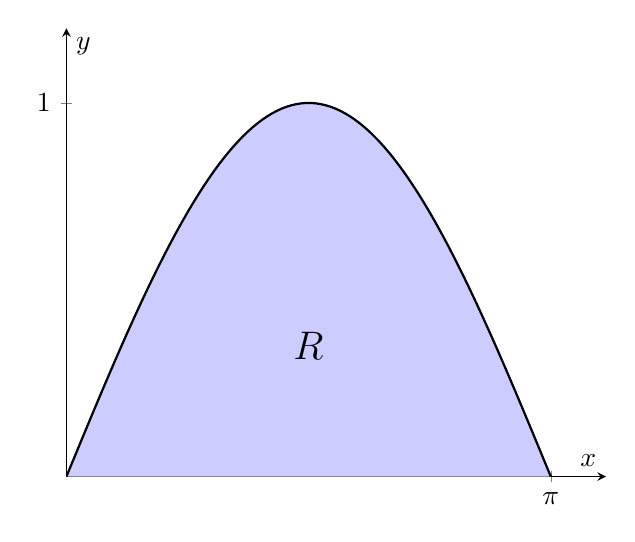
\begin{tikzpicture}
        \begin{axis}[
            axis lines = middle,
            xmin=0, xmax=3.5,
            ymin=0, ymax=1.2,
            xtick={0,3.14159},
            xticklabels={$0$,$\pi$},
            ytick={1},
            xlabel = {$x$},
            ylabel = {$y$},
        ]

        % Shade the region
        \addplot[
            domain=0:pi,
            samples=100,
            fill=blue!20,
            draw=none
        ] {sin(deg(x))} \closedcycle;

        % Draw sin(x)
        \addplot[
            domain=0:pi,
            samples=100,
            thick
        ] {sin(deg(x))};

        % R in the middle
        \node at (axis cs:1.57,0.35) {\Large $R$};

        \end{axis}
    \end{tikzpicture}
\end{figure}
\begin{equation*}
    \iint_R (x+y)^2\,dA
    =
    \int_0^{\pi}\int_0^{\sin(x)} (x+y)^2\,dy\,dx
\end{equation*}

hvor $dA$ betegner et infinitesimalt areal element i planet. Vi kan nu evaluere det indre integral med hensyn til $y$ helt som vi ville gøre med et normalt integral. Vi får:

\begin{equation*}
    \begin{aligned}
    \int_0^{\sin(x)} (x+y)^2\,dy
    &= \int_0^{\sin(x)} (x^2+2xy+y^2)\,dy \\
    &= \left[x^2y+xy^2+\frac{y^3}{3}\right]_0^{\sin(x)} \\
    &= x^2\sin(x)+x\sin^2(x)+\frac{\sin^3(x)}{3}
    \end{aligned}
\end{equation*}
Grænserne i dette integral skal forstås som, at hvis vi varierer $x$ fra 0 til $\pi$, så vil $y$ antage værdier der går fra 0 til $\sin(x)$.

Vi kan indsætte dette resultat tilbage i (1) og evaluere det ydre integral med hensyn til $x$:

\begin{equation*}
    \int_0^{\pi}
    \left(
    x^2\sin(x)
    +x\sin^2(x)
    +\frac{\sin^3(x)}{3}
    \right)\,dx
\end{equation*}

Dette kan opdeles i tre separate integraler:

\begin{equation*}
    \int_0^{\pi}x^2\sin(x)\,dx
    +
    \int_0^{\pi}x\sin^2(x)\,dx
    +
    \frac{1}{3}\int_0^{\pi}\sin^3(x)\,dx
\end{equation*}

De tre integraler kan evalueres ved hjælp af standard teknikker for integration, såsom partiel integration eller substitution. Resultaterne af disse integraler er:

\begin{equation*}
    \int_0^{\pi}x^2\sin(x)\,dx = \pi^2-4,
\end{equation*}

\begin{equation*}
    \int_0^{\pi}x\sin^2(x)\,dx = \frac{\pi^2}{4},
\end{equation*}

og

\begin{equation*}
    \int_0^{\pi}\sin^3(x)\,dx = \frac{4}{3}.
\end{equation*}

Vi kan derfor samle resultaterne:

\begin{equation*}
    \begin{aligned}
    \iint_R (x+y)^2\,dA
    &= (\pi^2-4)
    +\frac{\pi^2}{4}
    +\frac{1}{3}\left(\frac{4}{3}\right)\\
    &= \boxed{\frac{5\pi^2}{4}-\frac{32}{9}}.
    \end{aligned}
\end{equation*}

\end{document}
